%-------------------------------------------------------------------------------

% This file is part of Code_Saturne, a general-purpose CFD tool.
%
% Copyright (C) 1998-2012 EDF S.A.
%
% This program is free software; you can redistribute it and/or modify it under
% the terms of the GNU General Public License as published by the Free Software
% Foundation; either version 2 of the License, or (at your option) any later
% version.
%
% This program is distributed in the hope that it will be useful, but WITHOUT
% ANY WARRANTY; without even the implied warranty of MERCHANTABILITY or FITNESS
% FOR A PARTICULAR PURPOSE.  See the GNU General Public License for more
% details.
%
% You should have received a copy of the GNU General Public License along with
% this program; if not, write to the Free Software Foundation, Inc., 51 Franklin
% Street, Fifth Floor, Boston, MA 02110-1301, USA.

%-------------------------------------------------------------------------------

\programme{clsyvt}

\vspace{1cm}
%%%%%%%%%%%%%%%%%%%%%%%%%%%%%%%%%%
%%%%%%%%%%%%%%%%%%%%%%%%%%%%%%%%%%
\section*{Function}
%%%%%%%%%%%%%%%%%%%%%%%%%%%%%%%%%%
%%%%%%%%%%%%%%%%%%%%%%%%%%%%%%%%%%

The aim of this subroutine is to fill the arrays of boundary conditions 
 (\var{COEFA} and \var{COEFB}) of the velocity and of the Reynolds stress tensor,
for the symmetry boundary faces.
These conditions are express relatively naturally in the local coordinate system
of the boundary face. The function of \fort{clsyvt} is then to transform these 
natural boundary conditions (expressed in the local coordinate sytem) in the 
general coordinate sytem, and then to possibly partly implicit them. 

It should be noted that the part of the subroutine  \fort{clptur} (for the wall
boundary conditions) relative to the writing in the local coordinate system and to 
the rotation is totally identical.

%%%%%%%%%%%%%%%%%%%%%%%%%%%%%%%%%%
%%%%%%%%%%%%%%%%%%%%%%%%%%%%%%%%%%
\section*{Discretisation}
%%%%%%%%%%%%%%%%%%%%%%%%%%%%%%%%%%
%%%%%%%%%%%%%%%%%%%%%%%%%%%%%%%%%%

Figure \ref{Base_Clsyvt_fig_facesym} presents the notations used at the face. 
The local coordinate system is defined from the normal at the face and 
the velocity at $I'$ :\\
$\bullet\ \displaystyle\vect{t}
=\frac{1}{|\vect{u}_{I',\tau}|}\vect{u}_{I',\tau}$ is the first
vector of the local coordinate system.\\ 
$\bullet\ \vect{\tilde{n}}=-\vect{n}$ is the second
vector of the local coordinate system.\\ 
$\bullet\ \vect{b}=\vect{t}\wedge\vect{\tilde{n}}=\vect{n}\wedge\vect{t}$ 
is the third 
vector of the local coordinate system.\\

\begin{figure}[h]
\centerline{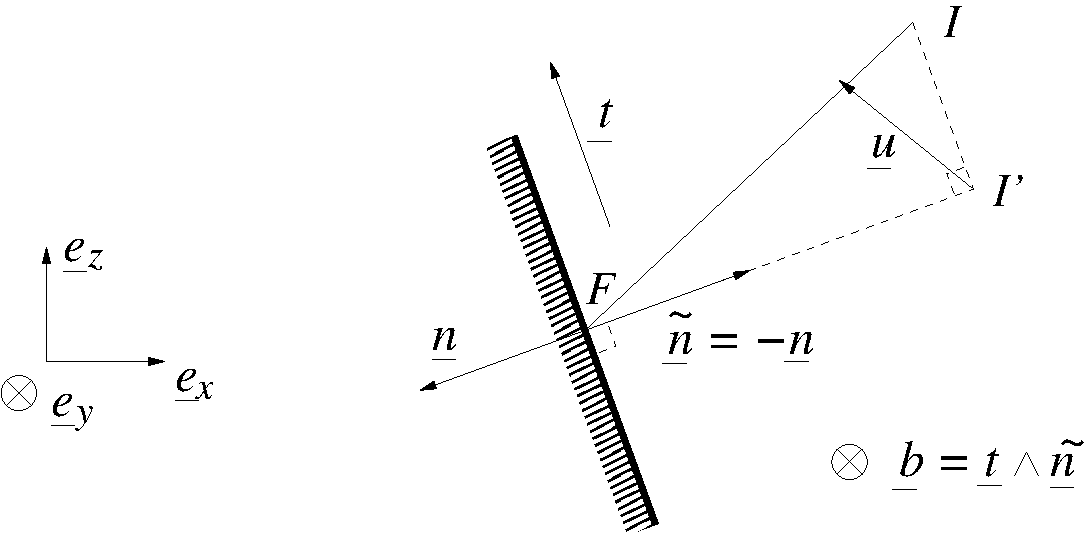
\includegraphics[width=8cm]{facesym}}
\caption{\label{Base_Clsyvt_fig_facesym}Definition of the vectors forming the local coordinate system.}
\end{figure}

Here, $\vect{n}$ is the normalized normal vector to the boundary face
in the sense of  \CS ({\em i.e.}
directed towards the outside of the computational domain) 
and $\vect{u}_{I',\tau}$ is the projection of the velocity at $I'$ 
in the plane of the face :
$\vect{u}_{I',\tau}=\vect{u}_{I'}-(\vect{u}_{I'}.\vect{n})\vect{n}$.\\
If $\vect{u}_{I',\tau}=\vect{0}$, the direction of $\vect{t}$ in the plane
normal to $\vect{n}$ is irrelevant. thus it is defined as :
$\displaystyle\vect{t}=\frac{1}{\sqrt{n_y^2+n_z^2}}(n_z\vect{e}_y-n_y\vect{e}_z)$
where
$\displaystyle\vect{t}=\frac{1}{\sqrt{n_x^2+n_z^2}}(n_z\vect{e}_x-n_x\vect{e}_z)$
along the non-zero components of $\vect{n}$ (components in the global
coordinate system $(\vect{e}_x,\vect{e}_y,\vect{e}_z)$).


For sake of clarity, the following notations will be used :\\
$\bullet\ $The general coordinate system will write 
$\mathcal{R}=(\vect{e}_x,\vect{e}_y,\vect{e}_z)$.\\
$\bullet\ $The local coordinate system will write
$\hat{\mathcal{R}}=(\vect{t},-\vect{n},\vect{b})=(\vect{t},\vect{\tilde{n}},\vect{b})$.\\
$\bullet\ $The matrices of the components of a vector $\vect{u}$ 
in the coordinate systems 
$\mathcal{R}$ and $\hat{\mathcal{R}}$ will write 
$\mat{U}$ and $\hat{\mat{U}}$, respectively.\\
$\bullet\ $The matrices of the components of a tensor $\tens{R}$ (2$^{nd}$ order) 
in the coordinate systems $\mathcal{R}$ and $\hat{\mathcal{R}}$ will write
 $\matt{R}$ and $\hat{\matt{R}}$, respectively.\\
$\bullet\ $ $\matt{P}$ refers to the (orthogonal) matrix transforming
 $\mathcal{R}$ into $\hat{\mathcal{R}}$.
\begin{equation}
\matt{P}=\left[
\begin{array}{ccc}
t_x & -n_x & b_x\\
t_y & -n_y & b_y\\
t_z & -n_z & b_z
\end{array}\right]
\end{equation}

($\matt{P}$ being orthogonal, $\matt{P}^{-1}=\,^t\matt{P}$).

In particular, we have for any vector $\vect{u}$
and for any second order tensor $\tens{R}$ :\\
\begin{equation}
\left\{\begin{array}{l}
\mat{U} = \matt{P}\,.\,\hat{\mat{U}}\\
\matt{R}= \matt{P}\,.\,\hat{\matt{R}}\,.\,^t\matt{P}
\end{array}\right.
\end{equation}

\minititre{Treatment of the velocity}
In the local coordinate system, the boundary conditions for $\vect{u}$ 
naturally write :\\
\begin{equation}
\left\{\begin{array}{lcl}
u_{F,t} & = & u_{I',t}\\
u_{F,\tilde{n}} & = & 0\\
u_{F,b} & = & u_{I',b}
\end{array}\right.
\end{equation}
or 
\begin{equation}
\mat{U}_F = \matt{P}\,.\,\hat{\mat{U}}_F
= \matt{P}\,.\,\left[
\begin{array}{ccc}
1 & 0 & 0\\
0 & 0 & 0\\
0 & 0 & 1
\end{array}
\right]\,.\,\hat{\mat{U}}_{I'}
=\matt{P}\,.\,\left[
\begin{array}{ccc}
1 & 0 & 0\\
0 & 0 & 0\\
0 & 0 & 1
\end{array}
\right]\,.\,^t\matt{P}\,.\,\mat{U}_{I'}
\end{equation}


Let's take 
$\matt{A}=\matt{P}\,.\,\left[
\begin{array}{ccc}
1 & 0 & 0\\
0 & 0 & 0\\
0 & 0 & 1
\end{array}
\right]\,.\,^t\matt{P}\qquad$ (matrix in the coordinate system $\mathcal{R}$ 
of the projector orthogonal to the face).

The boundary conditions for  $\vect{u}$ thus write :
\begin{equation}
\mat{U}_F = \matt{A}\,.\,\mat{U}_{I'}
\end{equation}

Since the matrix $\matt{P}$ is orthogonal, it can be shown that 
\begin{equation}
\matt{A}=\left[
\begin{array}{ccc}
1-\tilde{n}_x^2 & -\tilde{n}_x\tilde{n}_y & -\tilde{n}_x\tilde{n}_z\\
-\tilde{n}_x\tilde{n}_y & 1-\tilde{n}_y^2 & -\tilde{n}_y\tilde{n}_z\\
-\tilde{n}_x\tilde{n}_z & -\tilde{n}_y\tilde{n}_z & 1-\tilde{n}_z^2
\end{array}\right]
\end{equation}

The boundary conditions can then be partially implicited:
\begin{equation}
\label{Base_Clsyvt_eq_clU}
u_{F,x}^{(n+1)} = \underbrace{1-\tilde{n}_x^2}_{\var{COEFB}}u_{I',x}^{(n+1)}
\underbrace{-\tilde{n}_x\tilde{n}_y u_{I',y}^{(n)}
-\tilde{n}_x\tilde{n}_z u_{I',z}^{(n)}}_{\var{COEFA}}
\end{equation}

The other components have a similar treatment. Since only the coordinates 
of $\vect{n}$ are useful, we do not need (for $\vect{u}$) to define
explicitly the vectors  $\vect{t}$ and $\vect{b}$.

\vspace{1cm}
\minititre{Treatment of the Reynolds stress tensor}
We saw that we have the following relation:
\begin{equation}
\label{Base_Clsyvt_eq_chgtrepR}
\matt{R}= \matt{P}\,.\,\hat{\matt{R}}\,.\,^t\matt{P}
\end{equation}

The boundary conditions we want to write are relations of the type:
\begin{equation}
\comp{R}_{F,ij}=\sum_{k,l}\alpha_{ijkl}\comp{R}_{I',kl}
\end{equation}
We are then naturally brought to introduce the column matrices of the 
components of $\tens{R}$ in the different coordinate systems.

We write
\begin{equation}
\mat{S}=\,^t[\comp{R}_{11},\comp{R}_{12},\comp{R}_{13},
\comp{R}_{21},\comp{R}_{22},\comp{R}_{23},
\comp{R}_{31},\comp{R}_{32},\comp{R}_{33}]
\end{equation}
and
\begin{equation}
\hat{\mat{S}}=\,^t[\hat{\comp{R}}_{11},\hat{\comp{R}}_{12},\hat{\comp{R}}_{13},
\hat{\comp{R}}_{21},\hat{\comp{R}}_{22},\hat{\comp{R}}_{23},
\hat{\comp{R}}_{31},\hat{\comp{R}}_{32},\hat{\comp{R}}_{33}]
\end{equation}

Two functions $q$ and $r$ from $\{1,2,3,4,5,6,7,8,9\}$ to 
$\{1,2,3\}$ are defined. Their values are given in the following table :
\begin{center}
\begin{tabular}{|c|c|c|c|c|c|c|c|c|c|}
\hline
$i$&1&2&3&4&5&6&7&8&9\\
\hline
$q(i)$&1&1&1&2&2&2&3&3&3\\
\hline
$r(i)$&1&2&3&1&2&3&1&2&3\\
\hline
\end{tabular}
\end{center}
$i\longmapsto (q(i),r(i))$ is then a bijection from $\{1,2,3,4,5,6,7,8,9\}$
to $\{1,2,3\}^2$, and we have :
\begin{equation}
\left\{\begin{array}{l}
\comp{R}_{ij}=\comp{S}_{3(i-1)+j}\\
\comp{S}_i=\comp{R}_{q(i)r(i)}
\end{array}\right.
\end{equation}

Using equation \ref{Base_Clsyvt_eq_chgtrepR}, we thus have :
\begin{eqnarray}
\comp{S}_{F,i} & = & \comp{R}_{F,q(i)r(i)} =
\sum_{(m,n)\in\{1,2,3\}^2}\comp{P}_{q(i)m}\hat{\comp{R}}_{F,mn}\comp{P}_{r(i)n}\nonumber\\
&=&\sum_{j=1}^9\comp{P}_{q(i)q(j)}\hat{\comp{R}}_{F,q(j)r(j)}\comp{P}_{r(i)r(j)}
\quad\text{(d'apr\`es la bijectivit\'e de $(q,r)$)}\nonumber\\
&=&\sum_{j=1}^9\comp{P}_{q(i)q(j)}\comp{P}_{r(i)r(j)}\hat{\comp{S}}_{F,j}
\end{eqnarray}

Or 
\begin{equation}
\mat{S}_{F}=\matt{A}\,.\,\hat{\mat{S}}_F\quad\text{avec }
\comp{A}_{ij}=\comp{P}_{q(i)q(j)}\comp{P}_{r(i)r(j)}
\end{equation}

It can be shown that $\matt{A}$ is an orthogonal matrix (see Annexe A).


In the local coordinate system, the boundary conditions of $\tens{R}$
write naturally\footnote{cf. Davroux A., Archambeau F., {\em Le
$R_{ij}-\varepsilon$ dans \CS (version $\beta$)}, HI-83/00/030/A}.
\begin{equation}
\label{Base_Clsyvt_eq_clRij}%
\left\{\begin{array}{lll}
\hat{\comp{R}}_{F,11}=\hat{\comp{R}}_{I',11} \qquad\qquad&
\hat{\comp{R}}_{F,21}=0 \qquad\qquad&
\hat{\comp{R}}_{F,31}=B\hat{\comp{R}}_{I',31} \\
\hat{\comp{R}}_{F,12}=0 \qquad\qquad&
\hat{\comp{R}}_{F,22}=\hat{\comp{R}}_{I',22} \qquad\qquad&
\hat{\comp{R}}_{F,32}=0 \\
\hat{\comp{R}}_{F,13}=B\hat{\comp{R}}_{I',13} \qquad\qquad&
\hat{\comp{R}}_{F,23}=0 \qquad\qquad&
\hat{\comp{R}}_{F,33}=\hat{\comp{R}}_{I',33}
\end{array}\right.
\end{equation}

or
\renewcommand{\arraystretch}{0.5}
\begin{equation}
\hat{\mat{S}}_F=\matt{B}\,.\,\hat{\mat{S}}_{I'}
\qquad\text{avec }\matt{B}=
\left[\begin{array}{ccccccccc}
1&0&\cdots&\cdots&\cdots&\cdots&\cdots&\cdots&0\\
0&0&\ddots&&&&&&\vdots\\
\vdots&\ddots&B&\ddots&&&&&\vdots\\
\vdots&&\ddots&0&\ddots&&&&\vdots\\
\vdots&&&\ddots&1&\ddots&&&\vdots\\
\vdots&&&&\ddots&0&\ddots&&\vdots\\
\vdots&&&&&\ddots&B&\ddots&\vdots\\
\vdots&&&&&&\ddots&0&0\\
0&\cdots&\cdots&\cdots&\cdots&\cdots&\cdots&0&1
\end{array}\right]
\end{equation}
\renewcommand{\arraystretch}{1.}


For the symmetry faces which are treated by \fort{clsyvt}, the 
coefficient $B$ is 1. However a similar treatment is applied in
\fort{clptur} for the wall faces, and in this $B$ is zero. This 
parameter has to be specified when \fort{clca66} is called
(see \S\ref{Base_Clsyvt_prg_meo}).

Back in the global coordinate system, the following formulae is
finally obtained~:
\begin{equation}
\label{Base_Clsyvt_eq_clsurS}
\mat{S}_F=\matt{C}\,.\,\mat{S}_{I'}\qquad
\text{avec }\matt{C}=\matt{A}\,.\,\matt{B}\,.\,^t\matt{A}
\end{equation}

It can be shown that the components of the matrix $\matt{C}$ are :
\begin{equation}
\comp{C}_{ij}=\sum_{k=1}^9
\comp{P}_{q(i)q(k)}\comp{P}_{r(i)r(k)}\comp{P}_{q(j)q(k)}\comp{P}_{r(j)r(k)}
(\delta_{k1}+B\delta_{k3}+\delta_{k5}+B\delta_{k7}+\delta_{k9})
\end{equation}

To conclude, it can be noted that, due to the symmetries of the tensor  $\tens{R}$,
 the matrix $\mat{S}$. 
Thus only the simplified matrices 
$\mat{S}^\prime$ and $\hat{\mat{S}}^\prime$ will be used:
\begin{equation}
\mat{S}^\prime=\,^t[\comp{R}_{11},\comp{R}_{22},\comp{R}_{33},
\comp{R}_{12},\comp{R}_{13},\comp{R}_{23}]
\end{equation}
\begin{equation}
\hat{\mat{S}}^\prime=\,^t[\hat{\comp{R}}_{11},\hat{\comp{R}}_{22},\hat{\comp{R}}_{33},
\hat{\comp{R}}_{12},\hat{\comp{R}}_{13},\hat{\comp{R}}_{23}]
\end{equation}

By gathering different lines of matrix $\matt{C}$, equation 
\ref{Base_Clsyvt_eq_clsurS} is transformed into the final equation~:
\begin{equation}
\mat{S}_F^\prime=\matt{D}\,.\,\mat{S}_{I'}^\prime
\end{equation}

The computation of the matrix $\matt{D}$ is performed in the subroutine
\fort{clca66}. The methodology is described in annexe B.

From $\matt{D}$, the coefficients of the boundary conditions can be 
 partially implicited ($\var{ICLSYR}=1$) or totally explicited
($\var{ICLSYR}=0$).

$\bullet\ ${\sc Partial implicitation}\\
\begin{equation}
\label{Base_Clsyvt_eq_clRimp}
{\comp{S}_{F,i}^\prime}^{(n+1)} =
\underbrace{\comp{D}_{ii}}_{\var{COEFB}}{\comp{S}_{I',i}^\prime}^{(n+1)}
+\underbrace{\sum_{j\ne i}\comp{D}_{ij}{\comp{S}_{I',j}^\prime}^{(n)}}_{\var{COEFA}}
\end{equation}

$\bullet\ ${\sc Total explicitation}\\
\begin{equation}
\label{Base_Clsyvt_eq_clRexp}
{\comp{S}_{F,i}^\prime}^{(n+1)} =
\underbrace{\sum_j\comp{D}_{ij}{\comp{S}_{I',j}^\prime}^{(n)}}_{\var{COEFA}}
\qquad(\var{COEFB}=0)
\end{equation}

%%%%%%%%%%%%%%%%%%%%%%%%%%%%%%%%%%
%%%%%%%%%%%%%%%%%%%%%%%%%%%%%%%%%%
\section*{Implementation}
%%%%%%%%%%%%%%%%%%%%%%%%%%%%%%%%%%
%%%%%%%%%%%%%%%%%%%%%%%%%%%%%%%%%%
\label{Base_Clsyvt_prg_meo}%
\etape{Beginning of the loop}

Beginnning of the loop on all the boundary faces  \var{IFAC} with 
symmetry conditions.
A face is considered as a symmetry face if 
\var{ICODCL(IFAC,IU(IPHAS))} is 4. The tests in \fort{vericl} are designed 
 for  \var{ICODCL} to be equal to 4 for \var{IU} if and only if it is equal 
to 4 for the other components of the velocity and for the components of $\tens{R}$ 
(if necessary)\\.

The value 0 is given to  \var{ISYMPA}, which identifies the face as a 
wall or symmetry face (a face where the mass flux will be set to zero as 
explained in \fort{inimas}).

\etape{Calculation of the basis vectors}
The normal vector $\vect{n}$ is stored in \var{(RNX,RNY,RNZ)}.\\
$\vect{u}_{I'}$ is calculated in \fort{CONDLI}, passed {\em via} \var{COEFU},
and stored in \var{(UPX,UPY,UPZ)}.

\etape{Case with $R_{ij}-\varepsilon$}
With the $R_{ij}-\varepsilon$ model (\var{ITURB}=30 or 31), the vectors 
 $\vect{t}$ and $\vect{b}$ must be calculated explicitly
(we use $\matt{P}$, not simply $\matt{A}$).
They are stored in \var{(TX,TY,TZ)} and
\var{(T2X,T2Y,T2Z)}, respectively.\\
The transform matrix $\matt{P}$ is then calculated and stored in the array \var{ELOGLO}.\\
The subroutine \fort{clca66} is then called to calculate the reduced  
matrix $\matt{D}$. It is stored in \var{ALPHA}. \fort{clca66} is called 
with a parameter \var{CLSYME} which is 1, and which corresponds to the parameter
$\omega$ of equation \ref{Base_Clsyvt_eq_clRij}.


\etape{Filling the arrays \var{COEFA} and \var{COEFB}}
The arrays \var{COEFA} and \var{COEFB} are filled following directly
equations \ref{Base_Clsyvt_eq_clU}, \ref{Base_Clsyvt_eq_clRimp} and \ref{Base_Clsyvt_eq_clRexp}.\\
\var{RIJIPB(IFAC,.)} corresponds to the vector $\mat{S}_{I'}^\prime$, computed in 
\fort{condli}, and passed as an argument to \var{clsyvt}.

\etape{Filling the arrays \var{COEFAF} and \var{COEFBF}}
If they are defined, the arrays \var{COEFAF} and \var{COEFBF}
are filled. They contain the same values as \var{COEFA} and
\var{COEFB}, respectively.


%%%%%%%%%%%%%%%%%%%%%%%%%%%%%%%%%%
%%%%%%%%%%%%%%%%%%%%%%%%%%%%%%%%%%
\section*{Annexe A}
%%%%%%%%%%%%%%%%%%%%%%%%%%%%%%%%%%
%%%%%%%%%%%%%%%%%%%%%%%%%%%%%%%%%%
\minititre{Proof of the orthogonality of matrix $\matt{A}$}

All the notations used in paragraphe 2 are kept. We have :
\begin{eqnarray}
(^t\matt{A}\,.\,\matt{A})_{ij}
& = & \sum_{k=1}^9\comp{A}_{ki}\comp{A}_{kj}\nonumber\\
& = & \sum_{k=1}^9
\comp{P}_{q(k)q(i)}\comp{P}_{r(k)r(i)}\comp{P}_{q(k)q(j)}\comp{P}_{r(k)r(j)}
\end{eqnarray}
When $k$ varies from 1 to 3, $q(k)$ remains equal to 1 and $r(k)$ varies from 1
to 3. We thus have :
\begin{eqnarray}
\sum_{k=1}^3
\comp{P}_{q(k)q(i)}\comp{P}_{r(k)r(i)}\comp{P}_{q(k)q(j)}\comp{P}_{r(k)r(j)}
&=&\comp{P}_{1q(i)}\comp{P}_{1q(j)}\sum_{k=1}^3
\comp{P}_{r(k)r(i)}\comp{P}_{r(k)r(j)}\nonumber\\
&=&\comp{P}_{1q(i)}\comp{P}_{1q(j)}\sum_{k=1}^3
\comp{P}_{kr(i)}\comp{P}_{kr(j)}\\
&=&\comp{P}_{1q(i)}\comp{P}_{1q(j)}\delta_{r(i)r(j)}\qquad\text{(by
orthogonality of $\matt{P}$)}\nonumber
\end{eqnarray}
Likewise for $k$ varying from 4 to 6 or from 7 to 9, $q(k)$ being 2 or 3, respectively,
 we obtain :
\begin{eqnarray}
(^t\matt{A}\,.\,\matt{A})_{ij}
&=&
\sum_{k=1}^9
\comp{P}_{q(k)q(i)}\comp{P}_{r(k)r(i)}\comp{P}_{q(k)q(j)}\comp{P}_{r(k)r(j)}
\nonumber\\
&=&
\sum_{k=1}^3\comp{P}_{kq(i)}\comp{P}_{kq(j)}\delta_{r(i)r(j)}\\
&=&\delta_{q(i)q(j)}\delta_{r(i)r(j)}\nonumber\\
&=&\delta_{ij}\qquad
\text{(by the bijectivity of $(q,r)$)}\nonumber
\end{eqnarray}

Thus $^t\matt{A}\,.\,\matt{A}=\matt{Id}$. Similarly, it can be shown that 
$\matt{A}\,.\,^t\matt{A}=\matt{Id}$. Thus $\matt{A}$ is an orthogonal matrix.


%%%%%%%%%%%%%%%%%%%%%%%%%%%%%%%%%%
%%%%%%%%%%%%%%%%%%%%%%%%%%%%%%%%%%
\section*{Annexe B}
%%%%%%%%%%%%%%%%%%%%%%%%%%%%%%%%%%
%%%%%%%%%%%%%%%%%%%%%%%%%%%%%%%%%%
\minititre{Calculation of the matrix $\matt{D}$}

The relation between the matrices of dimension $9\times1$
of the components of $\tens{R}$ in the coordinate system $\mathcal{R}$ at $F$ and at $I'$
(matrices $\mat{S}_F$ and $\mat{S}_{I'}$) :
\begin{equation}
\mat{S}_F=\matt{C}\,.\,\mat{S}_{I'}
\end{equation}
with
\begin{equation}
\comp{C}_{ij}=\sum_{k=1}^9
\comp{P}_{q(i)q(k)}\comp{P}_{r(i)r(k)}\comp{P}_{q(j)q(k)}\comp{P}_{r(j)r(k)}
(\delta_{k1}+\omega\delta_{k3}+\delta_{k5}+\omega\delta_{k7}+\delta_{k9})
\end{equation}

To transform $\mat{S}$ into the matrix $6\times 1$ $\mat{S}^\prime$,
the function $s$ from $\{1,2,3,4,5,6,7,8,9\}$ to
$\{1,2,3,4,5,6\}$ is defined. It takes the following values :
\begin{center}
\begin{tabular}{|c|c|c|c|c|c|c|c|c|c|}
\hline
$i$&1&2&3&4&5&6&7&8&9\\
\hline
$s(i)$&1&4&5&4&2&6&5&6&3\\
\hline
\end{tabular}
\end{center}
By construction, we have $\comp{S}_i=\comp{S}^\prime_{s(i)}$ for all $i$ between 1
and 9.

To compute $\comp{D}_{ij}$, we can choose a value of $m$ to satisfy 
$s(m)=i$ and sum all the $\comp{C}_{mn}$ to have $s(n)=j$. The choice of $m$
is irrelevent. We can also compute the sum over all $m$ so that  $s(m)=i$ and then 
divide by the number of such values of $m$. We will use this method.

We define $N(i)$ the number of integers between 1 and 9 so that $s(m)=i$.
According to the preceeding, we thus have

\begin{eqnarray}
\comp{D}_{ij}&=&\frac{1}{N(i)}\sum_{s(m)=i \atop s(n)=j}\comp{C}_{mn}\nonumber\\
&=&\frac{1}{N(i)}\sum_{{s(m)=i \atop s(n)=j}\atop 1\leqslant k\leqslant 9}
\comp{P}_{q(m)q(k)}\comp{P}_{r(m)r(k)}\comp{P}_{q(n)q(k)}\comp{P}_{r(n)r(k)}
(\delta_{k1}+\omega\delta_{k3}+\delta_{k5}+\omega\delta_{k7}+\delta_{k9})
\end{eqnarray}

\vspace{1cm}
$\bullet\ ${\sc First case} : $i\leqslant 3$ and $j\leqslant 3$\\
In this case, we have $N(i)=N(j)=1$. Additionally, if $s(m)=i$ and $s(n)=j$,
then $q(m)=r(m)=i$ and $q(n)=r(n)=j$. Thus \\
\begin{equation}
\comp{D}_{ij}=\sum_{k=1}^9
\comp{P}_{iq(k)}\comp{P}_{ir(k)}\comp{P}_{jq(k)}\comp{P}_{jr(k)}
(\delta_{k1}+\omega\delta_{k3}+\delta_{k5}+\omega\delta_{k7}+\delta_{k9})
\end{equation}
When $k$ belongs to $\{1,5,9\}$, $q(k)=r(k)$ belongs to $\{1,2,3\}$. And for $k=3$ or
$k=7$, $q(k)=1$ and $r(k)=3$, or the inverse (and for $k$ even the 
the sum of Kronecker symbol is zero). Finally we have :
\begin{equation}
\comp{D}_{ij}=\sum_{k=1}^3\comp{P}_{ik}^2\comp{P}_{jk}^2
+2\omega\comp{P}_{j1}\comp{P}_{i3}\comp{P}_{i1}\comp{P}_{j3}
\end{equation}

\vspace{1cm}
$\bullet\ ${\sc Second case} : $i\leqslant 3$ and $j\geqslant 4$\\
Again we have $N(i)=1$, and if $s(m)=i$ then $q(m)=r(m)=i$.\\
On the contrary, we have $N(j)=2$, the two possibilities being $m_1$ and $m_2$.\\
\begin{itemize}
\item[-] if $j=4$, then $m_1=2$ and $m_2=4$,
$q(m_1)=r(m_2)=1$ and $r(m_1)=q(m_2)=2$. We then have
$m=1$ and $n=2$.

\item[-] if $j=5$, then $m_1=3$ and $m_2=7$,
$q(m_1)=r(m_2)=1$ and $r(m_1)=q(m_2)=3$. We then have
$m=1$ and $n=3$.

\item[-] if $j=6$, then $m_1=6$ and $m_2=8$,
$q(m_1)=r(m_2)=2$ and $r(m_1)=q(m_2)=3$. We then have 
$m=2$ and $n=3$.
\end{itemize}

And we have :
\begin{equation}
\comp{D}_{ij}=\sum_{k=1}^9
\comp{P}_{iq(k)}\comp{P}_{ir(k)}\left[
\comp{P}_{mq(k)}\comp{P}_{nr(k)}+\comp{P}_{nq(k)}\comp{P}_{mr(k)}\right]
(\delta_{k1}+\omega\delta_{k3}+\delta_{k5}+\omega\delta_{k7}+\delta_{k9})
\end{equation}

But when $k$ is in $\{1,5,9\}$, $q(k)=r(k)$ is in $\{1,2,3\}$. Thus :
\begin{equation}
\comp{D}_{ij}=2\sum_{k=1}^3
\comp{P}_{ik}^2\comp{P}_{mk}\comp{P}_{nk}
+\omega\sum_{k=1}^9
\comp{P}_{iq(k)}\comp{P}_{ir(k)}\left[
\comp{P}_{mq(k)}\comp{P}_{nr(k)}+\comp{P}_{nq(k)}\comp{P}_{mr(k)}\right]
(\delta_{k3}+\delta_{k7})
\end{equation}

And for $k=3$ or $k=7$, $q(k)=1$ and $r(k)=3$, or the opposite. We finally have :
\begin{equation}
\comp{D}_{ij}=2\left[\sum_{k=1}^3
\comp{P}_{ik}^2\comp{P}_{mk}\comp{P}_{nk}
+\omega\comp{P}_{i1}\comp{P}_{i3}\left(
\comp{P}_{m1}\comp{P}_{n3}+\comp{P}_{n1}\comp{P}_{m3}\right)
\right]
\end{equation}
with $(m,n)=(1,2)$ if $j=4$, $(m,n)=(1,3)$ if $j=5$ and $(m,n)=(2,3)$ if
$j=6$.

\vspace{1cm}
$\bullet\ ${\sc Third case} : $i\geqslant 4$ and $j\leqslant 3$\\
By symmetry of $\matt{C}$, we obtain a result which is the symmetric of
the second case, except that $N(i)$ is now 2. Thus :
\begin{equation}
\comp{D}_{ij}=\sum_{k=1}^3
\comp{P}_{jk}^2\comp{P}_{mk}\comp{P}_{nk}
+\omega\comp{P}_{j1}\comp{P}_{j3}\left(
\comp{P}_{m1}\comp{P}_{n3}+\comp{P}_{n1}\comp{P}_{m3}\right)
\end{equation}
with $(m,n)=(1,2)$ if $i=4$, $(m,n)=(1,3)$ if $i=5$ and $(m,n)=(2,3)$ if
$i=6$.

\vspace{1cm}
$\bullet\ ${\sc Fourth case} : $i\geqslant 4$ and $j\geqslant 4$\\
Then $N(i)=N(j)=2$.\\
We have $(m,n)=(1,2)$ if $i=4$, $(m,n)=(1,3)$ if $i=5$ and
$(m,n)=(2,3)$ if $i=6$. Likewise we define $m^\prime$ and
$n^\prime$ as a function of $j$. We then obtain :
\begin{eqnarray}
\comp{D}_{ij}&=&\frac{1}{2}\sum_{k=1}^9
\left(\comp{P}_{mq(k)}\comp{P}_{nr(k)}+\comp{P}_{nq(k)}\comp{P}_{mr(k)}\right)
\left(\comp{P}_{m^\prime q(k)}\comp{P}_{n^\prime r(k)}
+\comp{P}_{n^\prime q(k)}\comp{P}_{m^\prime r(k)}\right)\nonumber\\
&&\qquad\qquad\qquad\qquad\qquad\qquad\qquad\qquad\qquad\times
(\delta_{k1}+\omega\delta_{k3}+\delta_{k5}+\omega\delta_{k7}+\delta_{k9})\nonumber\\
&=&\frac{1}{2}\left[
\sum_{k=1}^3 4\comp{P}_{mk}\comp{P}_{nk}
\comp{P}_{m^\prime k}\comp{P}_{n^\prime k}
+2\omega\left(\comp{P}_{m1}\comp{P}_{n3}+\comp{P}_{n1}\comp{P}_{m3}\right)
\left(\comp{P}_{m^\prime 1}\comp{P}_{n^\prime 3}
+\comp{P}_{n^\prime 1}\comp{P}_{m^\prime 3}\right)\right]
\end{eqnarray}

and finally :
\begin{equation}
\comp{D}_{ij}=
2\sum_{k=1}^3  \comp{P}_{mk}\comp{P}_{nk}
\comp{P}_{m^\prime k}\comp{P}_{n^\prime k}
+\omega\left(\comp{P}_{m1}\comp{P}_{n3}+\comp{P}_{n1}\comp{P}_{m3}\right)
\left(\comp{P}_{m^\prime 1}\comp{P}_{n^\prime 3}
+\comp{P}_{n^\prime 1}\comp{P}_{m^\prime 3}\right)
\end{equation}
with $(m,n)=(1,2)$ if $i=4$, $(m,n)=(1,3)$ if $i=5$ and $(m,n)=(2,3)$ if
$i=6$\\
and $(m^\prime ,n^\prime )=(1,2)$ if $j=4$, $(m^\prime ,n^\prime )=(1,3)$
if $j=5$ and $(m^\prime ,n^\prime )=(2,3)$ if $j=6$.


